%% LyX 2.3.3 created this file.  For more info, see http://www.lyx.org/.
%% Do not edit unless you really know what you are doing.
\documentclass[12pt,english]{article}
\usepackage[T1]{fontenc}
\usepackage[latin9]{inputenc}
\usepackage{geometry}
\geometry{verbose,lmargin=1.5cm,rmargin=1.5cm}
\usepackage{array}
\usepackage{float}
\usepackage{graphicx}

\makeatletter

%%%%%%%%%%%%%%%%%%%%%%%%%%%%%% LyX specific LaTeX commands.
%% Because html converters don't know tabularnewline
\providecommand{\tabularnewline}{\\}

\@ifundefined{date}{}{\date{}}
\makeatother

\usepackage{babel}
\begin{document}
\title{Pollution Detection and Prediction System}

\maketitle
\noindent\begin{minipage}[t]{1\columnwidth}%
\begin{center}
\textbf{Project Report}
\par\end{center}%
\end{minipage}

\smallskip{}

\begin{center}
\textit{Submitted in partial fulfillment of the requirements for the }
\par\end{center}

\begin{center}
\textit{Degree of Bachelors in Engineering}
\par\end{center}

\vspace{1.5cm}

\begin{center}
\textit{by}
\par\end{center}

\noindent\begin{minipage}[t]{1\columnwidth}%
\begin{minipage}[t]{0.23\columnwidth}%
Rohit Martires

(Reg no. 1613032)%
\end{minipage}\hfill{}%
\begin{minipage}[t]{0.24\columnwidth}%
Swizel Monteiro

(Reg no. 1613033)%
\end{minipage}\hfill{}%
\begin{minipage}[t]{0.24\columnwidth}%
Vranda Asolkar

(Reg no. 1613001)%
\end{minipage}\hfill{}%
\begin{minipage}[t]{0.24\columnwidth}%
Vaylon Fernandes

(Reg no. 1613017)%
\end{minipage}%
\end{minipage}

\vspace{3cm}

\noindent\begin{minipage}[t]{1\columnwidth}%
\noindent\begin{minipage}[t]{1\columnwidth}%
\begin{center}
\textit{Under Guidance of}
\par\end{center}%
\end{minipage}

\medskip{}

\begin{center}
\begin{minipage}[t]{0.3\columnwidth}%
Dr. Shreyas Simu

(Internal Guide)%
\end{minipage}\hfill{}%
\begin{minipage}[t]{0.3\columnwidth}%
Dr. Varsha Turkar

(Internal Guide)%
\end{minipage}\hfill{}%
\begin{minipage}[t]{0.3\columnwidth}%
Mr. Vassant Salgaonkar

(External Guide)%
\end{minipage}
\par\end{center}%
\end{minipage}

\vspace{1cm}

\noindent\begin{minipage}[t]{1\columnwidth}%
\begin{center}
Electronics and Telecommunication
\par\end{center}%
\end{minipage}

\noindent\begin{minipage}[t]{1\columnwidth}%
\begin{center}
Don Bosco College Of Engineering
\par\end{center}%
\end{minipage}

\smallskip{}

\begin{center}
12/21/19
\par\end{center}

\newpage{}

\noindent\begin{minipage}[t]{1\columnwidth}%
\begin{center}
\textbf{ACKNOLEDGEMENT}
\par\end{center}%
\end{minipage}

\medskip{}

This project would not have been possible without the kind support
and help of many individuals and organizations. We would like to extend
our sincere thanks to all of them. 

We are highly indebted to Our Director, Rev. Fr. Kinley D\textquoteright Cruz
for providing us the necessary infrastructure to carry out our project
work with ease, Dr. Neena Panandikar, for giving us the opportunity
to work on this project.

We would like to express our gratitude to Dr. Varsha Turkar, Head
of Department of Electronics And Telecommunication Engineering and
Dr. Shreyas Simu project guides for their guidance and constant supervision
as well as for providing necessary information regarding the project
\& also for their support in completing the project.

We would like to thank Mr. Vassant Salgaonkar, our external guide
for his expert domain knowledge, kind co-operation, encouragement
and for giving us his time and attention.

Our thanks and appreciations also goes to all the faculty members
of Don Bosco College of Engineering for their expert advice and critical
guidance during various phases of our project. We also are in great
depth. to the ETC lab assistants, technical staff and librarian for
assisting us in building the project, and providing resources whenever
required by us for our project work.

Lastly, we place on records, a huge amount of thanks to Almighty,
our family and friends for their blessings, inspiration and constant
support and those who have helped us directly and indirectly for the
accomplishment of the project.

\newpage{}

\tableofcontents{}

\listoffigures

\listoftables

\newpage{}
\begin{abstract}
Industrial pollution is one of the most serious problems faced today.
Long term exposure to this pollution causes severe health issues including
respiratory and lung disorders. Presently laws regarding industrial
pollution monitoring and control are not stringent enough. But over
the years, Government of India is in the midst of making these laws
stricter. Hence, the proposed system aims at designing and building
a gadget that are durable in highly polluted climates and resistant
to a specified amount of temperature and pressure. The overall system
consists of network of sensors that will be mounted in a specific
industry, the data collected from these sensors will be stored on
the cloud using Internet Of Things (IOT). These sensors measure the
air parameters in terms of ambient air as well as stack emission.
On this data we apply various Machine Learning (ML) algorithms for
prediction of emission rate. From the study of various ML algorithms,
Kth Nearest Neighbours (KNN), Support Vector Regression (SVR), Random
Forest (RF), Multi linear regression (MLR) and Neural network (NN)
proved to have best results and hence were used. These algorithms
were implemented using python and the mean square error of each of
these was measured to check for accuracy and multi-linear perceptron
model was seen to have the least error. The air dispersion models
are then applied on the predicted emission rate to calculate the dispersion
of pollutants from the source that is at stack level. Based on the
study of various air dispersion models, the Gaussian model provides
the most optimal solution in terms of relatively low computational
time compared to others. The results were mapped onto a grayscale
bit mapped image where the pixel colour represents the concentration. 

\newpage{}
\end{abstract}

\section{INTRODUCTION}

With the rapid growth of the economy, industrial activities are increasing
more frequently, leading to a faster rate of pollution. This rate
is only increasing and if not kept in check can cause harmful effects
to mankind and other living organisms. These effects are amplified
if no regulation is kept in effect. Environmental pollution is one
of the most serious problems facing humanity and other life forms
on our planet today, industrial pollution contributing a major share
in it. Industrial pollution is generally referred to as the undesirable
outcome when factories or other industrial plants emit harmful by-products
and waste into the environment such as emissions into two main mediums
that are air and water. 

Air pollution constitutes of solid particles and gases which includes
dust, pollen and spores. Air pollutants can be largely classified
into 2 categories that is, primary pollutants that are usually produced
by processes that directly emit such as ash from volcanic eruption
or vehicle exhausts, and secondary pollutants that are both emitted
directly and formed from other primary pollutants such as photochemical
smog. 

Water pollution include contamination due to domestic wastes, insecticides
and herbicides, heavy metals and others, Such contamination can have
a wide range of adverse effects such as waterborne diseases, overgrowth
of toxic algae eaten by other aquatic animals and disruption of photosynthesis
in aquatic plants. 

The six major types of air pollutants are Carbon Monoxide (CO), Nitrogen
Oxides ($NO_{x}$), Sulphur Oxides ($SO_{x}$), particulates, hydrocarbons
and photochemical oxidants. 

\subsection{Project scope}

The Paris agreement\textquoteright s central aim is to strengthen
the global response to the threat of climate change by keeping a global
temperature rise this century well below 2 degrees Celsius above pre-industrial
levels \cite{falkner2016paris}. Long term exposure to polluted air
and water causes chronic health problems making the issue of industrial
pollution a severe one. It also lowers the air quality in surrounding
areas which causes many respiratory disorders affecting both lungs
and heart. Not just humans, but the marine life is greatly deteriorating
and affected with the extent of increasing industrial pollution. However,
with effective measures, the ill effect of industrial pollution could
be reduced significantly. The prevention and control of industrial
pollution are highly encouraged by the government worldwide. Simple
things like purchasing energy-efficient equipment and products made
from recycled materials, and having industrial pollution control policies
in place and strictly adhering to them. 

\subsection{Motivation}

The Draft Environment Laws (Amendment) Bill, 2015 was published by
the Ministry of Environment, Forest and Climate Change (MoEFCC) on
October 7, 2015. The objectives of the Draft Bill are to provide for
\textquotedblleft effective deterrent penal provisions\textquotedblright{}
i.e. a system that effectively punishes individuls, and to introduce
\textquotedblleft the concept of monetary penalty for violations and
contraventions\textquotedblright{} i.e. a sum of money imposed for
noncompliance. There are no effective strict rules for pollution monitoring
and control in industries yet. But the government of India is making
industrial pollution control and monitoring laws more strict.

\subsection{Objectives of the project}

The main objective of the project is to monitor the pollutants emitted
from an industry/factory and predict the future dispersion of these
pollutants also to then output these results in the form of reports
for industries/factories. To accomplish this project, three objectives
were identified that are
\begin{enumerate}
\item To create a series of gadgets which can measure the emission parameters
and the meteorological parameters and also that can withstand the
environmental conditions present near the stack/chimney and transmit
this information to a server that is Internet Of Things (IOT).
\item To develop a module that uses Machine Learning (ML) models with data
acquired from the cloud server to predict future emission parameter
values. 
\item To create a module that simulates the movement of fluid particles
(pollutant) in the air using air dispersion models with meteorological
data.
\end{enumerate}

\section{LITERATURE SURVEY}

In \cite{kaplan1996lagrangian} the authors proposed a diagnostic
model for calculating concentration distribution of a passive scalar
in a built-up area .This model basically requires measurements of
the wind velocity and direction at a certain reference height above
the obstacles. It is effectively able to predict 3-D concentration
distributions and is also able to identify concentration accumulation
at specific and precise points. It also succeeds in predicting concentration
distribution both quantitatively and qualitatively. The model can
be further used to study many air pollution phenomena.

\bigskip{}

The authors of \cite{de1998novel} proposed a detailed approach to
model dispersion which widely aims at combining the advantages of
puff models and particle models. The resulting model type is called
Puff-Particle Model (PPM). In PPM, hundred puffs in three dimensional
space is collectively simulated, in comparison to many thousand particles
usually required in pure particle models. The overall PPM concept
is quite simple, while puff growth is described by the concept of
relative dispersion which accounts for eddies smaller than the puff,
causing effect of meandering. The variation between the trajectories
of different puffs due to larger eddies, those larger than the actual
puff size is simulated by introducing puff-center trajectories derived
from particle trajectories from a particle model. 

\bigskip{}

In \cite{raza20023d} the authors proposed that the Lagrangian Monte
Carlo particle dispersion models works very effectively for the atmospheric
dispersion of effluents. It was also mentioned that in order to incorporate
the effect of vertical wind shear, the modified dispersion coefficient
should be used with the existing Gaussian plume model. As an alternative,
a much reliable 3D numerical model was used at a slightly greater
computational cost. This numerical model can also be used in a complex
topography region with hills and mountains, where mostly the conventional
Gaussian models seem to be less effective and mainly not suitable. 

\bigskip{}

The authors of \cite{li1996simplified} presented a model of (Nitrogen
Oxide) NO emissions for a power plant boiler. It was modelled from
the extended Zeldovich mechanism and it is observed that it requires
only a few physical parameters obtained from experiments. A set of
fresh new test data to compare the simulated values with real measurements
was used. It was observed that model performed well with real plant
input variables. The proposed model can also be used in other applications
such as for optimizing boiler operation and combustion control system
design.

\bigskip{}

In \cite{elshafei2006prediction} the authors proposed a model which
provided an efficient polynomial network solution to the problem of
tedious on-line monitoring of (Nitrogen Oxides) NOx emission from
industrial boilers. The effect of six variables was considered and
studied using 3D CFD simulation model and was used by polynomial networks
for prediction of NOx and Oxygen ($O_{2}$) in the exhaust flue. The
prediction of NOx and $O_{2}$ are both essential for efficient operation
and functioning of the boiler while maintaining the NOx pollutant
within a tolerable limit. The proposed soft sensor has a simple modular
structure for low cost implementation which is greatly an advantage.
This sensor can also be integrated with the boiler control system
for optimization of boilers operation increasing the effectiveness.

\bigskip{}

In \cite{yu2008pm} the authors presented a model, to study on the
factors to affect the Particulate Matter (PM-10) pollution and developed
a PM-10 prediction model using (Multi linear perceptron) MLP neural
network model. A neural model was used especially because it has an
advantage that there doesn\textquoteright t exist a need to analyze
the input data before the data are used, like that in regression model.
Also, to improve and optimize the performance of the proposed model
it required to shorten the learning period from year to quarter month
and to learn and predict PM-10 with multiple networks according to
the PM-10 levels.

\bigskip{}

The authors of \cite{xiaojun2015iot} proposed a good solution to
the complexity of air pollution. It was observed that use of a large
number of sensors ensures monitoring accuracy, greatly reduces monitoring
cost and makes monitoring data in monitoring area more perfect and
systematic. It was also noticed that addition of more meteorological
factors would highly improve the prediction performance. It used past
5 years data for training the model, showing that large sample data
can increase performance and train the model well. The overall experiment
used IOT and neural network for air pollution monitoring and forecasting.

\bigskip{}

The authors of \cite{yang2017new} proposed an Air quality monitoring
system with and an early warning system, including an assessment module
and a forecasting module. The model was able to successfully identify
the major pollutants in two cities. The experimental results showed
that the proposed model had the best accuracy and stability compared
to general regression neural network (GRNN), extended nearest neighbor
(ENN), MCSDE-ENN and MCSDE-EEMD-ENN.

\bigskip{}

In \cite{kang2018air} the authors compared research work on air quality
evaluation based on big data analytics, machine learning models and
techniques and also highlighted some future resource issues, needs
and challenges. It was stated that the accuracy of the air quality
evaluation and assessment is affected by device faults, battery issues
and sensor network. In this it was also mentioned that due to this
issue there is a strong need for research in data quality modelling
and automatic real-time validation. Also air in a city might be considered
as a multi-level air system. The need for research and development
of real-time air quality monitoring and evaluation and analysis on
multiple levels was also highlighted. It was said that smart cities
in the future must support real time air quality monitoring, evaluation
and prediction. This gives rise to the need to develop integrated
and dynamic air quality model using hybrid machine learning models.

\bigskip{}

The authors of \cite{ayele2018air} proposed a IOT based air quality
monitoring and prediction system. In this model sensor data of a humidity
and temperature sensor (DHT11) and a gas sensor (MQ135) was stored
on the cloud using a web-enabled microcontroller (ESP8266). This data
was then processed (converted into CSV) and used to train the machine
learning model and forecast the pollution rate. The machine learning
algorithm used is called Long Short Term Memory (LSTM) which is a
modification Recurrent Neural networks (RNN).

\bigskip{}

In \cite{zhu2018machine} the authors proposed refined models for
the prediction of hourly concentration of air pollution using meteorological
data of previous days by formulating the prediction over a 24 hour
period as a multi-task learning (MTL) problem. The results showed
that the proposed light formulation achieved the best result compared
to Baseline, and heavy formulation.

\bigskip{}

In \cite{delavar2019novel} the authors conducted a comparative study
of machine learning methods including nonlinear autoregressive exogenous
inputs (NARX), artificial neural network (ANN) and support vector
regression (SVR) which been employed for air pollution prediction
and the NARX was selected as the optimum one. The effective parameters
for air pollution prediction have been determined in this research.
This research used daily data of the pollutants. It also mentioned
that the quality of the proposed model can be significantly improved
if hourly data is implemented. Considering the importance of air pollution
problem, it was recommended that the number of air pollution measuring
stations increases so as to allow for a better fit on the air pollution
prediction. 

\bigskip{}

The authors of \cite{yi2018deep} proposed a DNN-based approach to
predict air quality. For this purpose a novel distributed fusion architecture
to fuse heterogeneous urban data was adopted, which could simultaneously
capture the individual and holistic effects from all influential factors
affecting air quality. This approach achieves a higher accuracy in
both general cases and sudden changes.

\bigskip{}

The authors of \cite{qu2009dynamic} developed a dynamic model to
estimate source emissions and predict contaminant concentration in
closed spaces. This was realized by using Extended Kalman Filter (EKF)
algorithm and least square method based on an established variable
--structural contaminant model. The model could realize to track
and real-time predict contaminant concentration, and identify source
emission rate accurately and efficiently.

\section{GAP ANALYSIS}

The previous work in this field included setting up monitoring stations
to measure the amount of pollutants in the atmosphere. This was done
using network of sensors topologically arranged as a grid \cite{xiaojun2015iot}.
These sensors are usually placed in a large area for e.g. around a
city or a large industry. The placement of sensors around a large
area can reduce the accuracy of the model. This happens because of
external factors like weather, noise, etc. affect the accuracy of
the sensors to a large extent. Also, these models can\textquoteright t
accurately reflect the extent of pollution a particular industry is
causing due to the large area. Some previous models also predicted
pollutant concentration for the future based on machine learning algorithms.
Also there were some models that predicted dispersion of pollutants
from a point source i.e. the area to which the pollutants will spread
to \cite{singh2018air}. No previous models have linked the emission
rate of the stack and the dispersion from the source(stack) together
i.e. they have not been predicting the emission rate and calculating
the spread in the same model.

The proposed model will however predict emission rate at the stack
and use it as a source to calculate dispersion using air dispersion
models. This will be done by placing sensors at the source (stack).
Placing the sensors at the source will help the sensors take more
accurate readings as the sensors will not be affected by external
factors to a large extent as compared to the previous models. This
will allow us to take more accurate readings and hence make more accurate
predictions of future emission rates.

\section{METHODOLOGY}

In Figure 1, methodology block diagram, the overall setup consists
of network of sensors that will be mounted in a specific industry,
the data collected from these sensors will be stored on the server.
These sensors measure the air parameters in terms of ambient air as
well as stack emission. On this data, we apply various machine learning
algorithms for prediction of emission rate. The air dispersion models
are then applied on the predicted emission rate to calculate the dispersion
of pollutants from the source that is at the stack level. The entire
system can be divided into two broad categories: IOT and ML

\begin{figure}[H]
\centering{}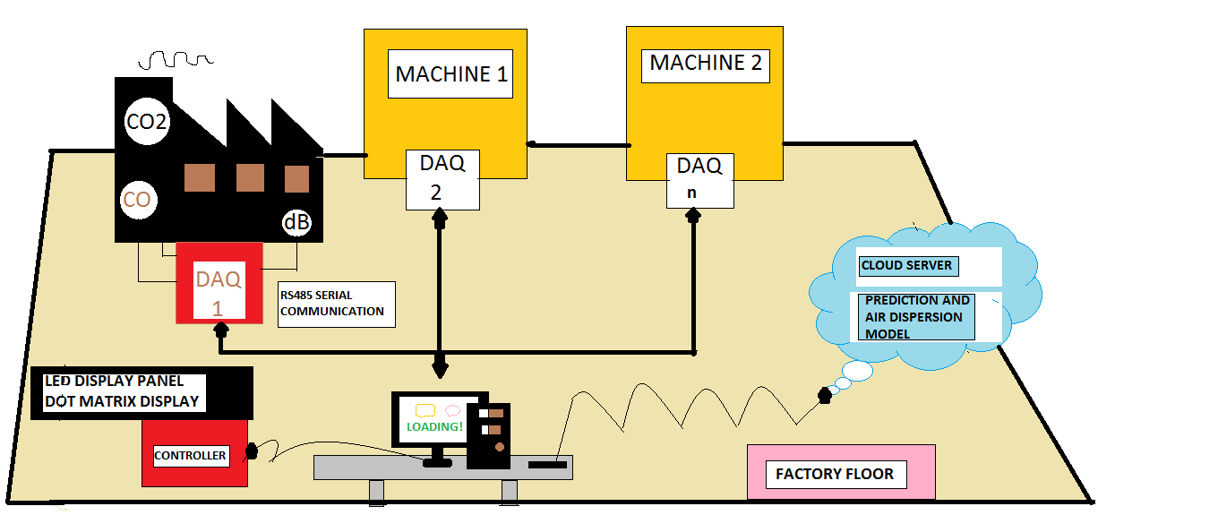
\includegraphics[width=10cm,height=10cm]{imgs/mainmeth}\caption{Methodology block diagram}
\end{figure}

\begin{figure}[H]
\begin{centering}
\includegraphics[width=13cm,height=13cm]{\string"imgs/iot process flow (1)\string".eps}
\par\end{centering}
\caption{IOT process flow}
\end{figure}

\begin{itemize}
\item \textbf{Internet Of Things:} in Figure 2, the IOT process flow begins
with air meteorological parameters, which are to be measured using
various sensors. On the basis of guidelines laid by central pollution
control board (CPCB), it is divided mainly into ambient air parameters
and stack emission parameters. 
\begin{itemize}
\item Ambient air parameters, refers to concentrations of pollutants in
the air, typically outdoor air. The criteria for this is based upon
protection of human health, crops, ecosystems as well as for planning
and other useful purposes. 
\item Stack emission parameters, parameters required to be monitored in
the stack emissions using continuous emission monitoring systems,
are industry specific. 
\item Consideration of parameters to predict emission rate (Q) and Velocity
of wind (V), we considered all the air meteorological parameters inorder
to predict the value of V and Q. 
\item Data collection using sensors, with the help of various sensors employed
in a specific industry, huge amount of data was collected. 
\item Building up of cloud architecture, the data collected from the sensors
is uploaded and stored on the cloud setup. The sensor network is connected
to the cloud server. 
\end{itemize}
\end{itemize}
\begin{figure}[H]
\centering{}\includegraphics[width=13cm,height=13cm]{\string"imgs/ML process flow (1)\string".eps}\caption{Machine Leaning process flow}
\end{figure}

\begin{itemize}
\item \textbf{Machine Learning}: in Firgure 3, the machine learning process
flow begins with 
\begin{itemize}
\item Dummy data is generated using python. The dummy data was not truly
random, it was correlated with various meteorological air parameters
so that the machine could be trained well. It was observed that by
adding more meteorological factors, the prediction performance is
greatly improved and large sample data can improve performance and
train the model well.
\item Implementation of ML algorithms, machine learning algorithms were
then implemented on the created dummy data to predict the value of
'Q' emission rate and 'V' velocity of wind. For this purpose, the
data was divided into training set (80\%) and test set (20\%). If
the error reduces for training as well as test data, the process is
continued. Else if the error reduces only for training data, but increases
for test data then the process is terminated. This could greatly increase
chances of generalizability of the algorithm. 
\item Performance check, was then conducted on the predicted emission rate.
The mean square error was measured in each case to check for accuracy. 
\item Optimization of algorithms, various algorithms were optimized in such
a way so as to reduce the error as minimum as possible thereby increasing
the accuracy of prediction. On this basis, the best algorithm was
selected. 
\item We chose Gaussian dispersion model to calculate dispersion and the
extent of pollution spread since it was the most optimal model in
terms of computing power. 
\item Prediction of air pollution, in this manner the entire process of
prediction of pollution and calculation of its spread is done.
\end{itemize}
\end{itemize}

\subsection{Machine Learning Algorithms }

Based on previous work the various machine learning algorithms were
compared based on the pollutants considered, accuracy, simplicity,
robustness, flexibility, sensors used, and other factors that affect
the choice of models. The following proved to have best results hence
these were used:- 
\begin{enumerate}
\item \textbf{Kth Nearest Neighbors (KNN)-} In this machine learning model
similar things are considered to be in close proximity to each other.
The value of K indicates the nearest neighbors that are taken for
consideration. This similarity criterion can be based on distance
or other similar factors. It uses a database that is separated into
several classes to predict the classification of a new sample point.
It is extended as a regression technique wherein the output of the
point is the average or median value of its nearest neighbors. In
KNN the training data required is very less, which means there is
a lack of generalization {[}17{]}. 
\item \textbf{Support Vector Regression (SVR)-} SVR is a supervised machine
learning algorithm that is being used for both classification and
regression problems. In this algorithm, a data point is plotted in
n-dimensional space after which it is classified by finding the plane
that will differentiate the classes very well. The hyperplane which
is considered is a linear separator of any dimension (line, plane,
hyperplane). The training points are used in decision function and
are called support vectors {[}18{]}.
\item \textbf{Random Forest (RFS)-} The decision tree is a decision support
tool. It uses a graph in the form of a tree to show possible consequences.
Random forest operates by constructing multiple decision trees during
the training phase. The decision of the majority of the trees is chosen
by the random forest as the final decision. When a training data set
is considered with targets and features, some set of rules are formulated,
these rules are used to perform predictions. It identifies the most
important features out of all the available features in the training
dataset. The larger the no. of trees the more accurate the results
will be. Random forest classifier handles missing values and overfitting
problem doesn\textquoteright t exist {[}19{]}.
\item \textbf{Multilinear Regression (MLR)-} This technique uses several
explanatory variables to predict the outcome of the response variable.
A linear relationship is modeled between these independent and response
variable (dependent). Prediction about one variable is done based
on the information about the other variable. In this case, the independent
variables should not be too highly correlated with each other {[}20{]}.
\item \textbf{Neural Network (MLP)-} it is a model that mimics the way the
human brain operates. A neuron in a neural network is a mathematical
function that collects and classifies information according to some
specific architecture. A neural network contains layers of interconnected
nodes. Each connection is associated with a weight that is multiplied
with the input value. Each neuron has an activation function that
defines the output of the neuron which is used to introduce non-linearity
in the network model {[}21{]}.
\end{enumerate}
These Machine learning algorithms were implemented using python and
the mean square error of each of these was measured to check for accuracy.

\subsection{Air Dispersion Model}

\subsubsection{Gaussian Dispersion Model }

Gaussian dispersion model \cite{singh2018air} is a steady-state system,
the concentration of pollution downwind from a source is treated as
spreading outward from the stack. A point source was considered somewhere
in the air where a pollutant is released at a constant rate Q (kg/s).
The wind is blowing continuously in a direction x (measured in meters
from the source) with a speed U (m/s). The plume spreads as it moves
in the x-direction such that the local concentrations C(x,y,z) (kg/m3)
at any point in space form distributions which have shapes that are
Gaussian or normal in planes normal to the x-direction i.e. the concentration
of the pollution will be maximum at the source and will gradually
disperse where this dispersion follows a gaussian curve. The maximum
concentration is in the direction of the wind and there will be lateral
dispersion on the y-z plane. The more the dispersion area, the more
diluted will be the pollutant. 

\subsubsection{Lagrangian Model }

The Lagrangian model determines the trajectory of air pollutants.
The pollutants are tracked as air parcels which move along trajectories
determined by wind field, the buoyancy and turbulence effects. The
trajectory calculations are based on ordinary differential equations(ODE)
instead of partial differential equations which are used in the gaussian
dispersion model. The estimation of the concentration field is given
by the final distribution of a large number of particles. The particles
can be tracked from the source area to the area of reception. The
computational cost of these models is independent of the output grid
resolution and hence they are very efficient for short-range modeling.
For long-range simulations, however, the computational cost increases
as there is a need to calculate a large number of single trajectories.
Also, a large amount of computational power is required to handle
a large number of puffs.

\subsubsection{Puff-Plume Model }

The puff-plume model maintains the advantages of the puff models and
also of the plume models. The pollutant particles are grouped in clusters.
These clusters are treated as Gaussian puffs which are dispersed using
the concept of relative diffusion. The center of mass of each puff
follows a stochastic trajectory. The particle trajectories of the
Lagrangian stochastic dispersion model gives the trajectory of the
puffs.

\subsubsection{Why Gaussian model?}

The Gaussian dispersion model has been selected as it has relatively
less computational time as compared to the Lagrangian model in which
the computational time increases significantly with an increase in
distance. 

\subsection{Dataset and study area}

The objective of the prediction module is to predict the emission
rate at the stack/chimney. To build and test the prediction model,
1000 dummy data points were generated using Gaussian distribution
to randomly generate values for the feature set with guidance from
an industry expert, this data was later split into training and testing
that is 80\% and 20\% respectively. The feature set is chosen on the
basis of what factors will correlate to the emission rate and the
type of pollutants emitted from the stack. The feature set consists
of independent variables: day, month, type of industry, size of the
industry, and output efficiency of industry and dependent variable:
emission rate.
\begin{itemize}
\item Type of industry: what the industry/factory produces which will correlate
to what gases are emitted out of the stack/chimney, this will be in
the form of labeled classes. 
\item Size of the industry: how big is the industry/factory which will correlate
how much the maximum is outputted, this will be represented in the
form of a scale from 1 to 10.
\item Output efficiency: the amount of output it produces each day divided
by the total amount of output it can ideally produce. 
\item Emission rate: this is defined as the amount of pollutants released
from the stack per unit time.
\end{itemize}
The prediction module is also used on the collected meteorological
data to predict the air velocity and direction, this is then applied
to calculate the dispersion of pollutants in the air.

The feature set of this prediction model consists of independent variables:
day, month, ambient temperature, ambient pressure, moisture content
and dependent variables: the air velocity and air direction.

Day and month are used to timestamp data points also temperature,
pressure and moisture content of the ambient air is correlated to
the velocity and direction of air.

\section{RESULTS}

The prediction module and air dispersion module was implemented in
python programing language using Spyder Integrated development environment.

The prediction module was tested on the dummy data set generated then
the precision was measured by finding the deviation of the predicted
value from the actual value using mean square error. In an attempt
to optimize the models the parameters of the models were tuned and
the response (mean squared error) was graphed out.

The air dispersion module was implemented to calculate the concentration
from a stationary steady state point source i.e. stack and the results
were mapped onto a grayscale bitmap image where the pixel color represents
the concentration. 

\subsection{Machine Learning module}

Different Machine Learning algorithms were studied and implemented
on the same dataset and the results were compared. Table 1: shows
the range of error in the respective models while the parameters were
tuned

\smallskip{}

\begin{table}[H]
\begin{centering}
\begin{tabular}{|c|>{\centering}p{4cm}|>{\raggedright}p{3cm}|>{\centering}p{1.5cm}|>{\centering}p{1cm}|>{\centering}p{1cm}|}
\hline 
Sr no. & Name of ML model & Parameters & Min error $\frac{m}{hr}^{3}$

\smallskip{}
 & Max error $\frac{m}{hr}^{3}$ & Avg. error $\frac{m}{hr}^{3}$\tabularnewline
\hline 
\hline 
1 & Random Forest & maximum depth

maximum features

minimum sample split

minimum sample leaf

n estimators & 5 & 24 & 14.5\tabularnewline
\hline 
2 & Multi-linear perceptron regression & activation function

number of neurons

solvers & 2.2 & 2.7 & 2.45\tabularnewline
\hline 
3 & Support vector regression & kernel & 10 & 10.8 & 10.4\tabularnewline
\hline 
4 & K-nearest neighbor & weight

algorithm & 3 & 14 & 8.5\tabularnewline
\hline 
5 & Multi-linear Regression & None & 10 & 10 & 10\tabularnewline
\hline 
\end{tabular}
\par\end{centering}
\caption{Comparison of ML algorithms}
\end{table}

\pagebreak{}

The following graphs shows the mean square error while the parameters
are being tuned for the respective models

\subsubsection{Random forest (RF):}

The random forest model was tuned on its parameters that are 
\begin{itemize}
\item N estimators: The number of trees in the forest. 
\item Maximum depth: The maximum depth of the tree. 
\item Minimum samples split: The minimum number of samples required to split
an internal node. 
\item Minimum samples leaf: The minimum number of samples required to be
at a leaf node. 
\item Maximum features: he number of features to consider when looking for
the best split. 
\end{itemize}
\begin{figure}[H]
\centering{}%
\begin{minipage}[t]{0.45\columnwidth}%
\begin{center}
\includegraphics[width=6.5cm,height=6.5cm,keepaspectratio]{\string"readings/random forest/max_depth\string".eps}\caption{Parameter tuned max depth}
\par\end{center}%
\end{minipage}\hfill{}%
\begin{minipage}[t]{0.45\columnwidth}%
\begin{center}
\includegraphics[width=6.5cm,height=6.5cm,keepaspectratio]{\string"readings/random forest/max_features\string".eps}\caption{Parameter tuned max features}
\par\end{center}%
\end{minipage}
\end{figure}

\begin{figure}[H]
\centering{}%
\begin{minipage}[t]{0.45\columnwidth}%
\begin{center}
\includegraphics[width=6.5cm,height=6.5cm,keepaspectratio]{\string"readings/random forest/minsapmleaf\string".eps}\caption{Parameter tuned min sample leaf}
\par\end{center}%
\end{minipage}\hfill{}%
\begin{minipage}[t]{0.45\columnwidth}%
\begin{center}
\includegraphics[width=6.5cm,height=6.5cm,keepaspectratio]{\string"readings/random forest/minsapmsplit\string".eps}\caption{Parameter tuned min sample split}
\par\end{center}%
\end{minipage}
\end{figure}

\begin{figure}[H]
\begin{centering}
\includegraphics[width=6.5cm,height=6.5cm,keepaspectratio]{\string"readings/random forest/n_estimators\string".eps}
\par\end{centering}
\caption{Parameter tuned n estimators}
\end{figure}

As shown in Figure 4,5,6,7 and 8 that tuning the 'N estimators', 'max
features' and 'max depth' doesn\textquoteright t vary the error by
any significant value but tuning 'min sample leaf' and 'min sample
split' does impact the error.

\subsubsection{Multi-linear perceptron (MLP) regression: }

Here the model is tuned on 
\begin{itemize}
\item Activation: Activation function for the hidden layer. 
\item Solver: The solver for weight optimization. 
\item Number of neurons: the number of neurons used in the hidden layer. 
\end{itemize}
\begin{figure}[H]
\centering{}%
\begin{minipage}[t]{0.45\columnwidth}%
\begin{center}
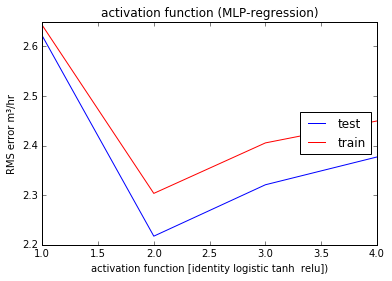
\includegraphics[width=6.5cm,height=6.5cm,keepaspectratio]{readings/mlp/actfunc}\caption{Parameter tuned activation function}
\par\end{center}%
\end{minipage}\hfill{}%
\begin{minipage}[t]{0.45\columnwidth}%
\begin{center}
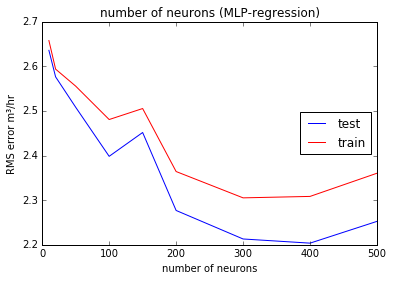
\includegraphics[width=6.5cm,height=6.5cm,keepaspectratio]{readings/mlp/noofnue}\caption{Parameter tuned number of neurons}
\par\end{center}%
\end{minipage}
\end{figure}

\begin{figure}[H]
\centering{}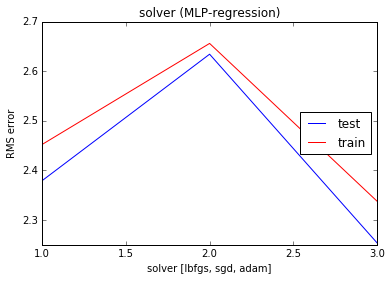
\includegraphics[width=6.5cm,height=6.5cm,keepaspectratio]{readings/mlp/solver}\caption{Parameter tuned solver}
\end{figure}

Figure 9,10 and 11 shows that after tuning activation function, number
of neurons and type of solvers the error change is lies between 2.2
and 2.6 which is not too significant

\subsubsection{Support vector regression (SVR):}

This model is only tuned on 
\begin{itemize}
\item Kernel: Specifies the kernel type to be used in the algorithm.
\end{itemize}
\begin{figure}[H]
\centering{}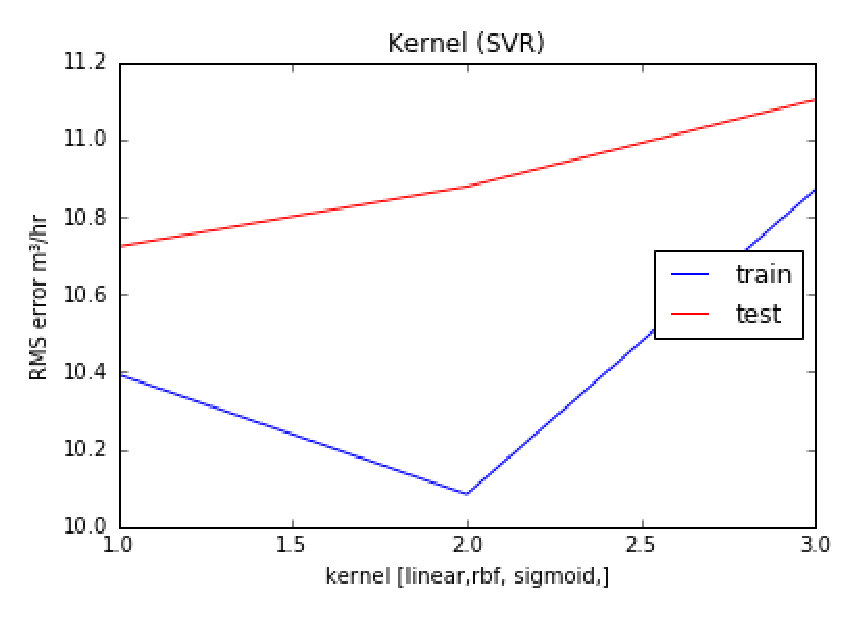
\includegraphics[width=6.5cm,height=6.5cm,keepaspectratio]{readings/svm/kernel}\caption{Parameter tuned kernel}
\end{figure}

Figure 12 shows that the SVR model was tuned on its kernel property
and the following results show that the rbf kernel had the least error

\subsubsection{K-nearest neighbor (KNN):}

This was tuned on 
\begin{itemize}
\item Weights: weight function used in prediction. 
\item Algorithm: Algorithm used to compute the nearest neighbors. 
\end{itemize}
\begin{figure}[H]
\centering{}%
\begin{minipage}[t]{0.45\columnwidth}%
\begin{center}
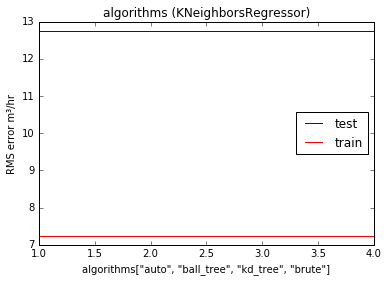
\includegraphics[width=6.5cm,height=6.5cm,keepaspectratio]{readings/knn/knn_algo}
\par\end{center}
\begin{center}
\caption{Parameter tuned algorithm}
\par\end{center}%
\end{minipage}\hfill{}%
\begin{minipage}[t]{0.45\columnwidth}%
\begin{center}
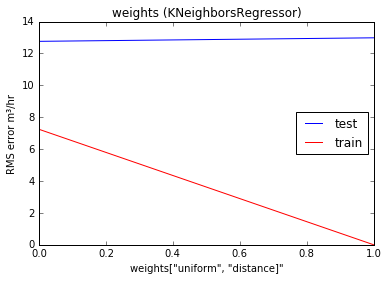
\includegraphics[width=6.5cm,height=6.5cm,keepaspectratio]{readings/knn/knn_weights}\caption{Parameter tuned weights}
\par\end{center}%
\end{minipage}
\end{figure}

Figure 13 and 14 show that the KNN model was tuned on its algorithm
and weight parameter used to cluster data points, the results shows
that varying both these parameters does not change the error by any
significant amount

\subsubsection{Multi-linear Regression (MLR):}

This algorithm is an extension of linear regression with added support
of higher dimensions in feature space

\begin{figure}[H]
\centering{}%
\begin{minipage}[t]{0.45\columnwidth}%
\begin{center}
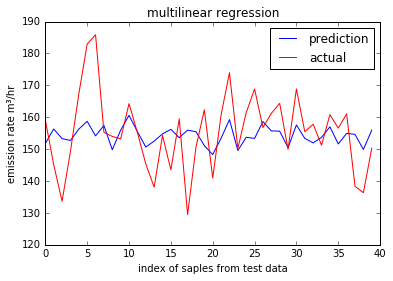
\includegraphics[width=6.5cm,height=6.5cm,keepaspectratio]{readings/mlr/mlp_testdata}\caption{Model tested on testing data}
\par\end{center}%
\end{minipage}\hfill{}%
\begin{minipage}[t]{0.45\columnwidth}%
\begin{center}
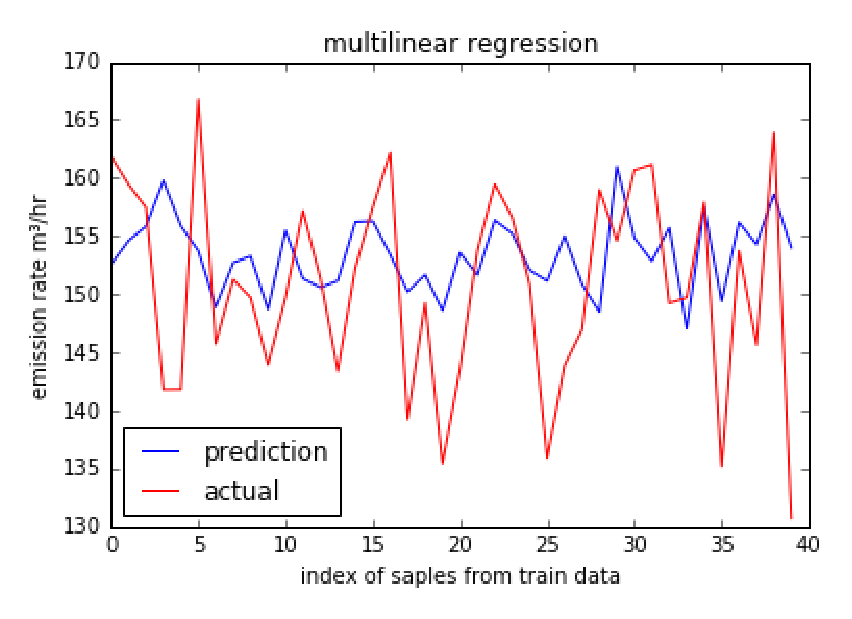
\includegraphics[width=7cm,height=7cm,keepaspectratio]{readings/mlr/mlp_traindata}\caption{Model tested on trainig data}
\par\end{center}%
\end{minipage}
\end{figure}

The above results in Figure 15 and 16 shows that the plot of predicted
value and actual value, the predicted values closely follows the actual
values with an average error of about 10$m^{3}/hr$

\bigskip{}

The results of the prediction module clearly shows that the multi-perceptron
regression model has the least mean square error out of all the models
also we can see that the error using test data loosely follows the
error using training data i.e. the area between both plots over parameter
tuning does not change much which is a good indication that overfitting
is not occurring. Whereas multi-linear regression has the most error
due to its simplistic design.

\subsection{Air Dispersion module}

To calculate the concentration of the pollutant after emission from
the stack, Gaussian air dispersion model was used for simulation,
this was implemented using python programing language. The results
were then represented using a thresholding functions to map different
concentration levels with a color level, and this was outputted as
an image.

\begin{figure}[H]
\centering{}\includegraphics[width=9cm,height=9cm,keepaspectratio]{\string"readings/gaussian disp model/result\string".eps}\caption{Gaussian air dispersion model}
\end{figure}

Figure 17, shows the diffrent levels of concentration, white color
represents regions with high concentration and black with low concentration.

\section{CONCLUSION}

The pollution detection and prediction system which was divided into
3 main objectives, out of which 2 were successfully implemented that
is 
\begin{itemize}
\item Air dispersion module: in the module the Gaussian air dispersion model
was implemented using python in spyder IDE. 
\item Prediction module: in this module 5 machine learning models were implemented
and compared which include (Random forest, Multi-linear perceptron,
K-nearest neighbor, Support vector regression, Multi-linear regression)
from these Multi-linear perceptron model was seen to have the least
error.
\end{itemize}
\newpage{}

\bibliographystyle{ieeetr}
\addcontentsline{toc}{section}{\refname}\bibliography{citations/working,\string"citations/Exported Items\string"}

\noindent\begin{minipage}[t]{1\columnwidth}%
{[}17{]} A. Bronshtein, \textquotedblleft A Quick Introduction to
K-Nearest Neighbors Algorithm,\textquotedblright{} Medium, 06-May-2019.
{[}Online{]}. Available: https://blog.usejournal.com/a-quick-introduction-to-k-nearest-neighbors-
algorithm-62214cea29c7. {[}Accessed: 13-Jan-2020{]}.

\medskip{}

{[}18{]} I. Bhattacharyya, \textquotedblleft Support Vector Regression
Or SVR,\textquotedblright{} Medium, 12-Jul-2018. {[}Online{]}. Available:
https://medium.com/coinmonks/support-vector-regression-or-svr-8eb3acf6d0ff.
{[}Accessed: 13-Jan-2020{]}.

\medskip{}

{[}19{]} \textquotedblleft Understanding Random Forest - Towards Data
Science.\textquotedblright{} {[}Online{]}. Available: https://towardsdatascience.com/understanding-random-forest-58381e0602d2.
{[}Accessed: 13-Jan-2020{]}.

\medskip{}

{[}20{]} W. Kenton, \textquotedblleft How Multiple Linear Regression
Works,\textquotedblright{} Investopedia. {[}Online{]}. Available:
https://www.investopedia.com/terms/m/mlr.asp. {[}Accessed: 13-Jan-2020{]}.

\medskip{}

{[}21{]} \textquotedblleft Neural Networks Explained - Data Driven
Investor - Medium.\textquotedblright{} {[}Online{]}. Available: https://medium.com/datadriveninvestor/neural-networks-explained-6e21c70d7818.
{[}Accessed: 13-Jan-2020{]}.%
\end{minipage}
\end{document}
